\usetikzlibrary{arrows.meta}
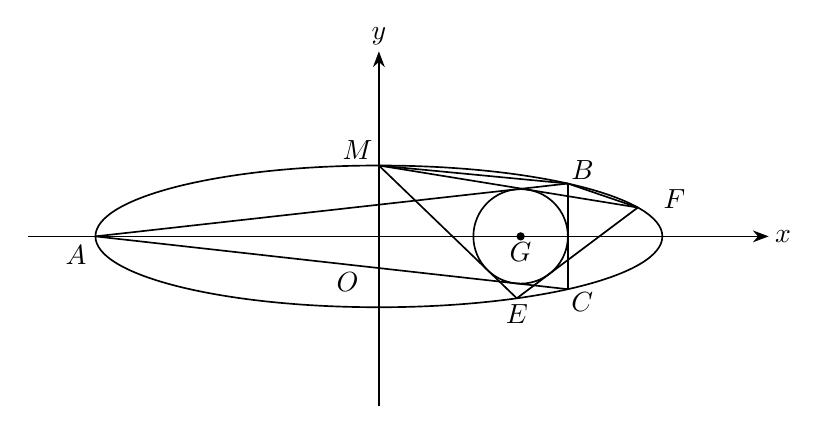
\begin{tikzpicture}[x=1cm,y=1cm,line width=.6pt,>={Stealth},font=\normalsize]
\coordinate (O) at (0,0);
\coordinate (A) at (-3.6,0);
\coordinate (B) at (2.4,0.67082);
\coordinate (C) at (2.4,-0.67082);
\coordinate (M) at (0,0.9);
\coordinate (G) at (1.8,0);
\coordinate (E) at (1.751625,-0.786282);
\coordinate (F) at (3.288375,0.366282);
\draw[->] (-4.45,0) -- (4.95,0) node[right,inner sep=0pt,xshift=2pt] {$x$};
\draw[->] (0,-2.15) -- (0,2.35) node[above,inner sep=0pt,yshift=2pt] {$y$};
\draw (O) ellipse[x radius=3.6cm,y radius=0.9cm];
\draw (G) circle[radius=0.6cm];
\draw (A) -- (B);
\draw (A) -- (C);
\draw (B) -- (C);
\draw (M) -- (B);
\draw (M) -- (F);
\draw (M) -- (E);
\draw (E) -- (F);
\draw (B) -- (F);
\fill (G) circle[radius=1.5pt];
\node[below left,inner sep=3pt] at (A) {$A$};
\node[above right,inner sep=0pt,xshift=1pt,yshift=1pt] at (B) {$B$};
\node[below right,inner sep=0pt,xshift=1pt,yshift=-1pt] at (C) {$C$};
\node[above left,inner sep=0pt,xshift=-2pt,yshift=2pt] at (M) {$M$};
\node[right,inner sep=0pt,xshift=9pt,yshift=3pt] at (F) {$F$};
\node[below,inner sep=0pt,yshift=-2pt] at (E) {$E$};
\node[below,inner sep=0pt,yshift=-2pt] at (1.8,0) {$G$};
\node[below left,inner sep=0pt] at (-0.25,-0.45) {$O$};
\end{tikzpicture}
